%%% LaTeX Template: Newsletter
%%%
%%% Source: http://www.howtotex.com/
%%% Feel free to distribute this template, but please keep the referal to HowToTeX.com.
%%% Date: September 2011


%%% ---------------
%%% PREAMBLE
%%% ---------------
\documentclass[10pt,a4paper]{article}

% Define geometry (without using the geometry package)
\setlength\topmargin{-48pt}
\setlength\headheight{0pt}
\setlength\headsep{25pt}
\setlength\marginparwidth{-20pt}
\setlength\textwidth{7.0in}
\setlength\textheight{9.5in}
\setlength\oddsidemargin{-30pt}
\setlength\evensidemargin{-30pt}

\frenchspacing						% better looking spacing

% Call packages we'll need
\usepackage[english]{babel}			% english
\usepackage{graphicx}				% images
\usepackage{amssymb,amsmath}		% math
\usepackage{multicol}				% three-column layout
\usepackage{url}					% clickable links
\usepackage{marvosym}				% symbols
\usepackage{wrapfig}				% wrapping text around figures
\usepackage[T1]{fontenc}			% font encoding
\usepackage{charter} 				% Charter font for main content
\usepackage{blindtext}				% dummy text
\usepackage{datetime}				% custom date
	\newdateformat{mydate}{\monthname[\THEMONTH] \THEYEAR}
\usepackage[pdfpagemode=FullScreen,
			colorlinks=false]{hyperref}	% links and pdf behaviour

% Customize (header and) footer
\usepackage{fancyhdr}
\pagestyle{fancy}
\fancyhf{}
\lfoot{	\footnotesize 
		Newletter from HowToTeX.com \\
		\Mundus\ \href{http://www.howtotex.com}{HowToTeX.com}	\quad
		\Telefon\ 555-5555											\quad
		\Letter\ \href{mailto:frits@howtotex.com}{frits@howtotex.com}
	  }
\cfoot{}
\rfoot{\footnotesize ~\\ Page \thepage}
\renewcommand{\headrulewidth}{0.0pt}	% no bar on top of page
\renewcommand{\footrulewidth}{0.4pt}	% bar on bottom of page

%%% ---------------
%%% DEFINITIONS
%%% ---------------

% Define separators
\newcommand{\HorRule}[1]{\noindent\rule{\linewidth}{#1}} % Creating a horizontal rule
\newcommand{\SepRule}{\noindent							 % Creating a separator
						\begin{center}
							\rule{250pt}{1pt}
						\end{center}
						}						

% Define Title en News input
\newcommand{\JournalName}[1]{%
		\begin{center}	
			\Huge \usefont{T1}{augie}{m}{n}
			#1%
		\end{center}	
		\par \normalsize \normalfont}
		
\newcommand{\JournalIssue}[1]{%
		\hfill \textsc{\mydate \today, No #1}
		\par \normalsize \normalfont}

\newcommand{\NewsItem}[1]{%
		\usefont{T1}{augie}{m}{n} 	
		\large #1 \vspace{4pt}
		\par \normalsize \normalfont}
		
\newcommand{\NewsAuthor}[1]{%
			\hfill by \textsc{#1} \vspace{4pt}
			\par \normalfont}		

\newcommand\sect[1]{%
  \section*{#1}%
  \addcontentsline{toc}{section}{#1}}

\newcommand{\HRule}{\rule{\linewidth}{0.5mm}}


%%% ---------------
%%% BEGIN DOCUMENT
%%% ---------------
\begin{document}



\begin{titlepage}

\begin{center}


% Upper part of the page
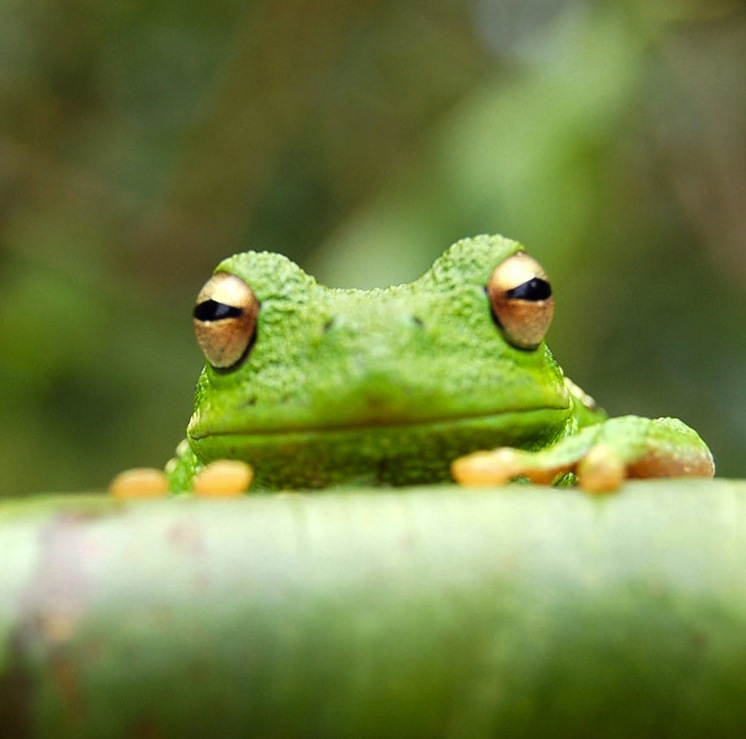
\includegraphics[width=0.15\textwidth]{frog.jpg}\\[1cm]    

\textsc{\LARGE University of Beer}\\[1.5cm]

\textsc{\Large Final year project}\\[0.5cm]


% Title
\HRule \\[0.4cm]
{ \huge \bfseries Lager brewing techniques}\\[0.4cm]

\HRule \\[1.5cm]

% Author and supervisor
\begin{minipage}{0.4\textwidth}
\begin{flushleft} \large
\emph{Author:}\\
John \textsc{Smith}
\end{flushleft}
\end{minipage}
\begin{minipage}{0.4\textwidth}
\begin{flushright} \large
\emph{Supervisor:} \\
Dr.~Mark \textsc{Brown}
\end{flushright}
\end{minipage}

\vfill

% Bottom of the page
{\large \today}

\end{center}

\end{titlepage}


% Title	
% -----
\JournalIssue{1}
\JournalName{Explorers Club of Pittsburgh}
\noindent\HorRule{3pt} \\[-0.75\baselineskip]
\HorRule{1pt}
% -----

\tableofcontents

% Front article
% -----
\vspace{0.5cm}
	\SepRule
\vspace{0.5cm}



\begin{center}
\begin{minipage}[h]{0.75\linewidth}
	\begin{wrapfigure}{l}{0.41\textwidth}
		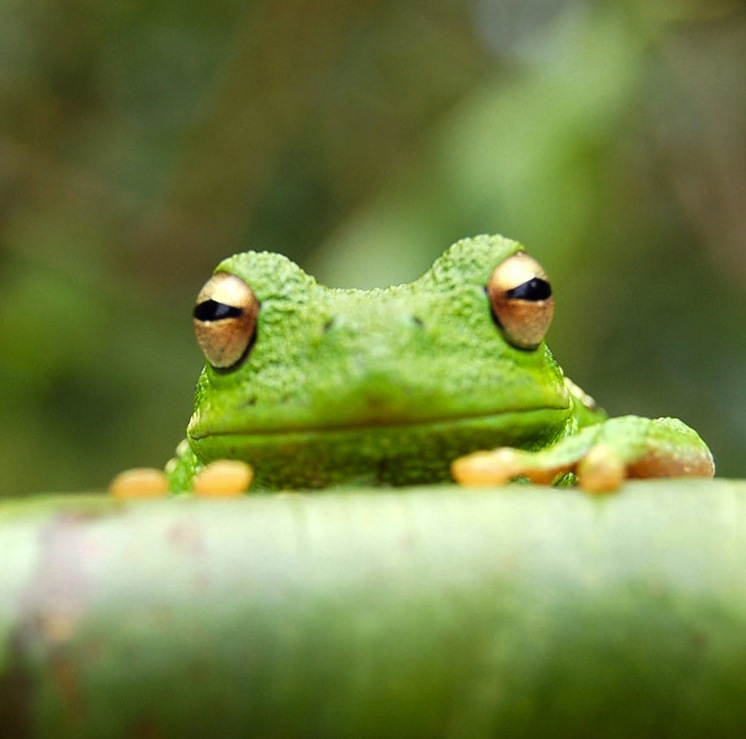
\includegraphics[width=0.42\textwidth]{frog.jpg}
		\\	% this spacer is needed to make the text on the right fit OK
	\end{wrapfigure}
	
	\NewsItem{Frog eats monkey}
	\emph{\blindtext}
\end{minipage}
\end{center}
% -----



% Other news (1)
% -----
\vspace{0.5cm}
	\SepRule
\vspace{0.5cm}
\begin{multicols}{2}

\sect{Section 1}

	\NewsItem{Monkey eats elephant}
	\NewsAuthor{F. Wenneker}
	\blindtext[2] 
% -----

\sect{Section2}

\vspace{1cm}
% Other news (2)
% -----
\NewsItem{Elephant eats frog}
\NewsAuthor{J. Doe}
	\blindtext[1]
		\begin{center}
			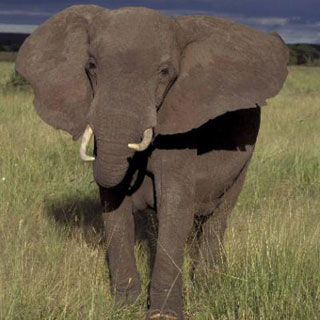
\includegraphics[width=0.8\linewidth]{elephant}
		\end{center}
		\blindtext[1]





\end{multicols}
% -----


%---
\section*{What a wonderful world}
This is such a wonderful document

%----
\end{document} 

